% Copyright (c)) 2014,2016 Casper Ti. Vecto
% Public domain
\chapter{系統需求分析}

透過特性要因分析可以將比特幣的交易监督系统大致分為四個主題,如圖\ref{fish1}所示,分別為信息安全技術、加密貨幣錢包、近場通訊技術以及數據庫。作為⼀個⾦流系統,四項主軸之中信息安全是不可或缺的環節,著重於商家認證機制、用戶權限控管、身份識別管理、使用者訪問控制四個方向;本系統致力於奠定匿名對實名的加密貨幣系統,必須對區塊鏈技術、公鑰私鑰生成算法、點對點交易技術、錢包地址產出以及貨幣發行技術五個方向進行探討;在交易場景中,本系統採用近場通信技術,因此需要對商品RFID標籤建置、讀取商品RFID標籤以及Android Beam傳輸商品交易進行基礎的API調研;為了使加密貨幣實名制的實現,數據庫必須存儲與政府和商家相關的信息。此時數據庫加密、個人信息去識別化安全以及數據庫連接便相當重要。
		\begin{figure}[!htbp]
			\centering
			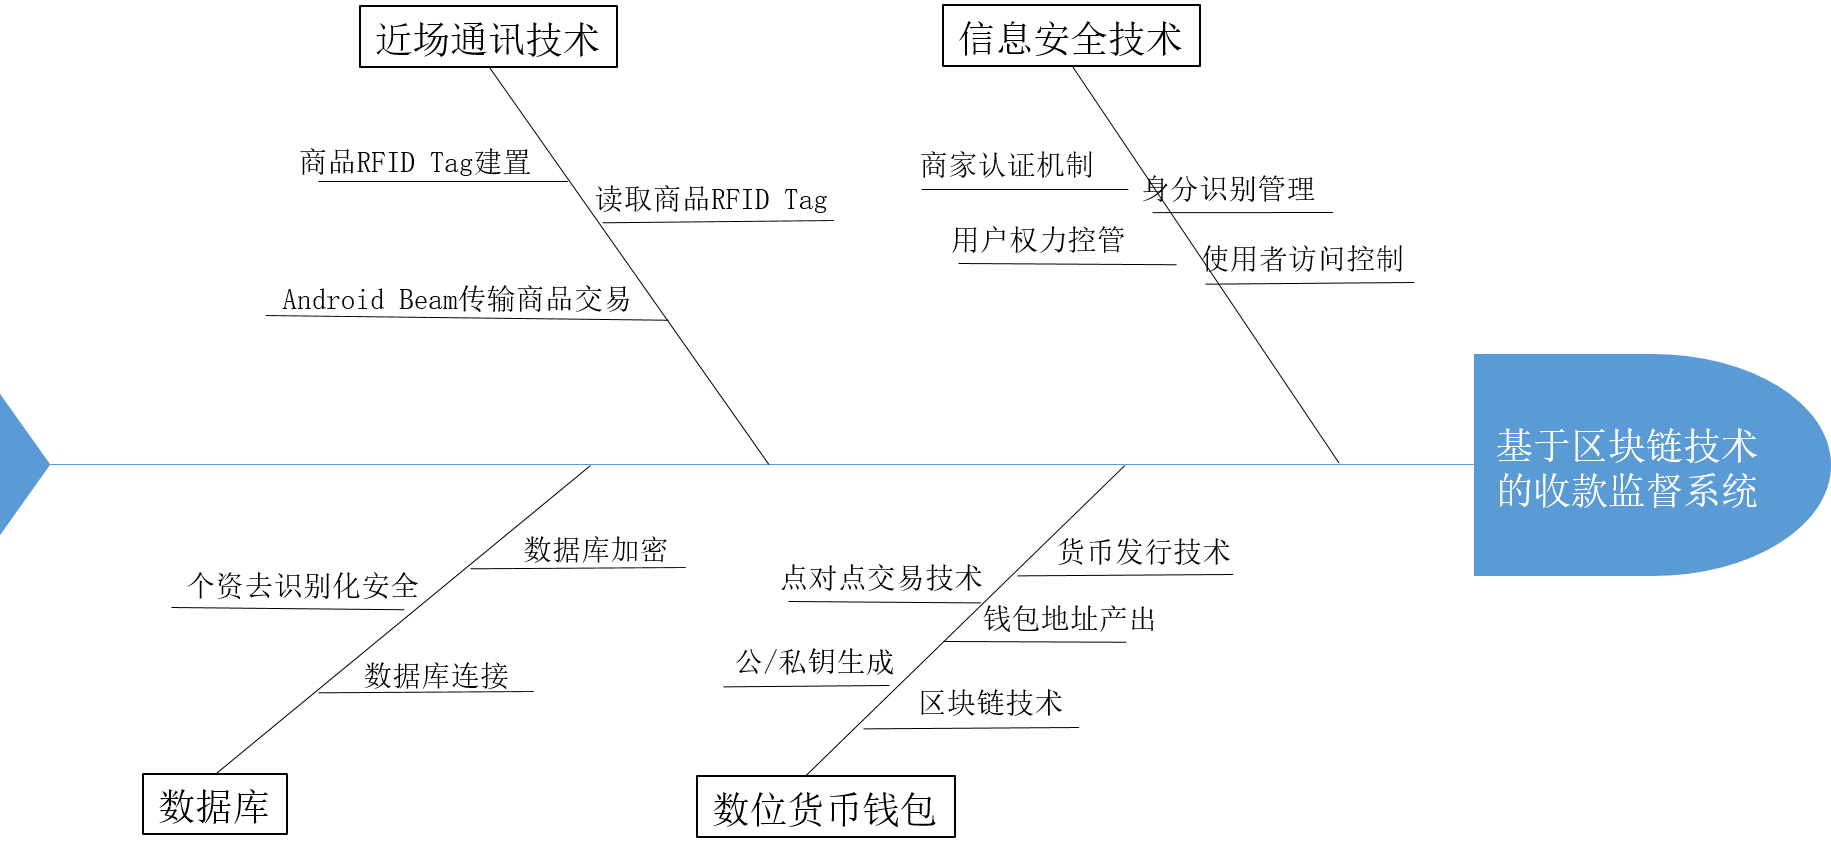
\includegraphics[width = 0.8\textwidth]{fish1.png}
			\caption{⽐特幣的交易监督系統特性要因分析圖}\label{fish1}
		\end{figure}

為了使本⽂所提出的系統設計之模塊更加明確,對系統進⾏詳細的需求分析可以使應確⽴的⽅向更加分明,在本章將分為三節進行分析,分別為交易模型分析、功能性需求分析以及非功能性需求分析。


\section{交易模型分析}

在設計比特幣的监督系统之前必須針對現今社會中人與人之間的交易方式進行分析,在支付的方式依照使用人數比例大致可區分為現金交易以及電子支付兩種類別,圖\ref{modeall}為各種交易模型示意圖。
%%fig allan
\begin{figure}[!htbp]
	\centering
	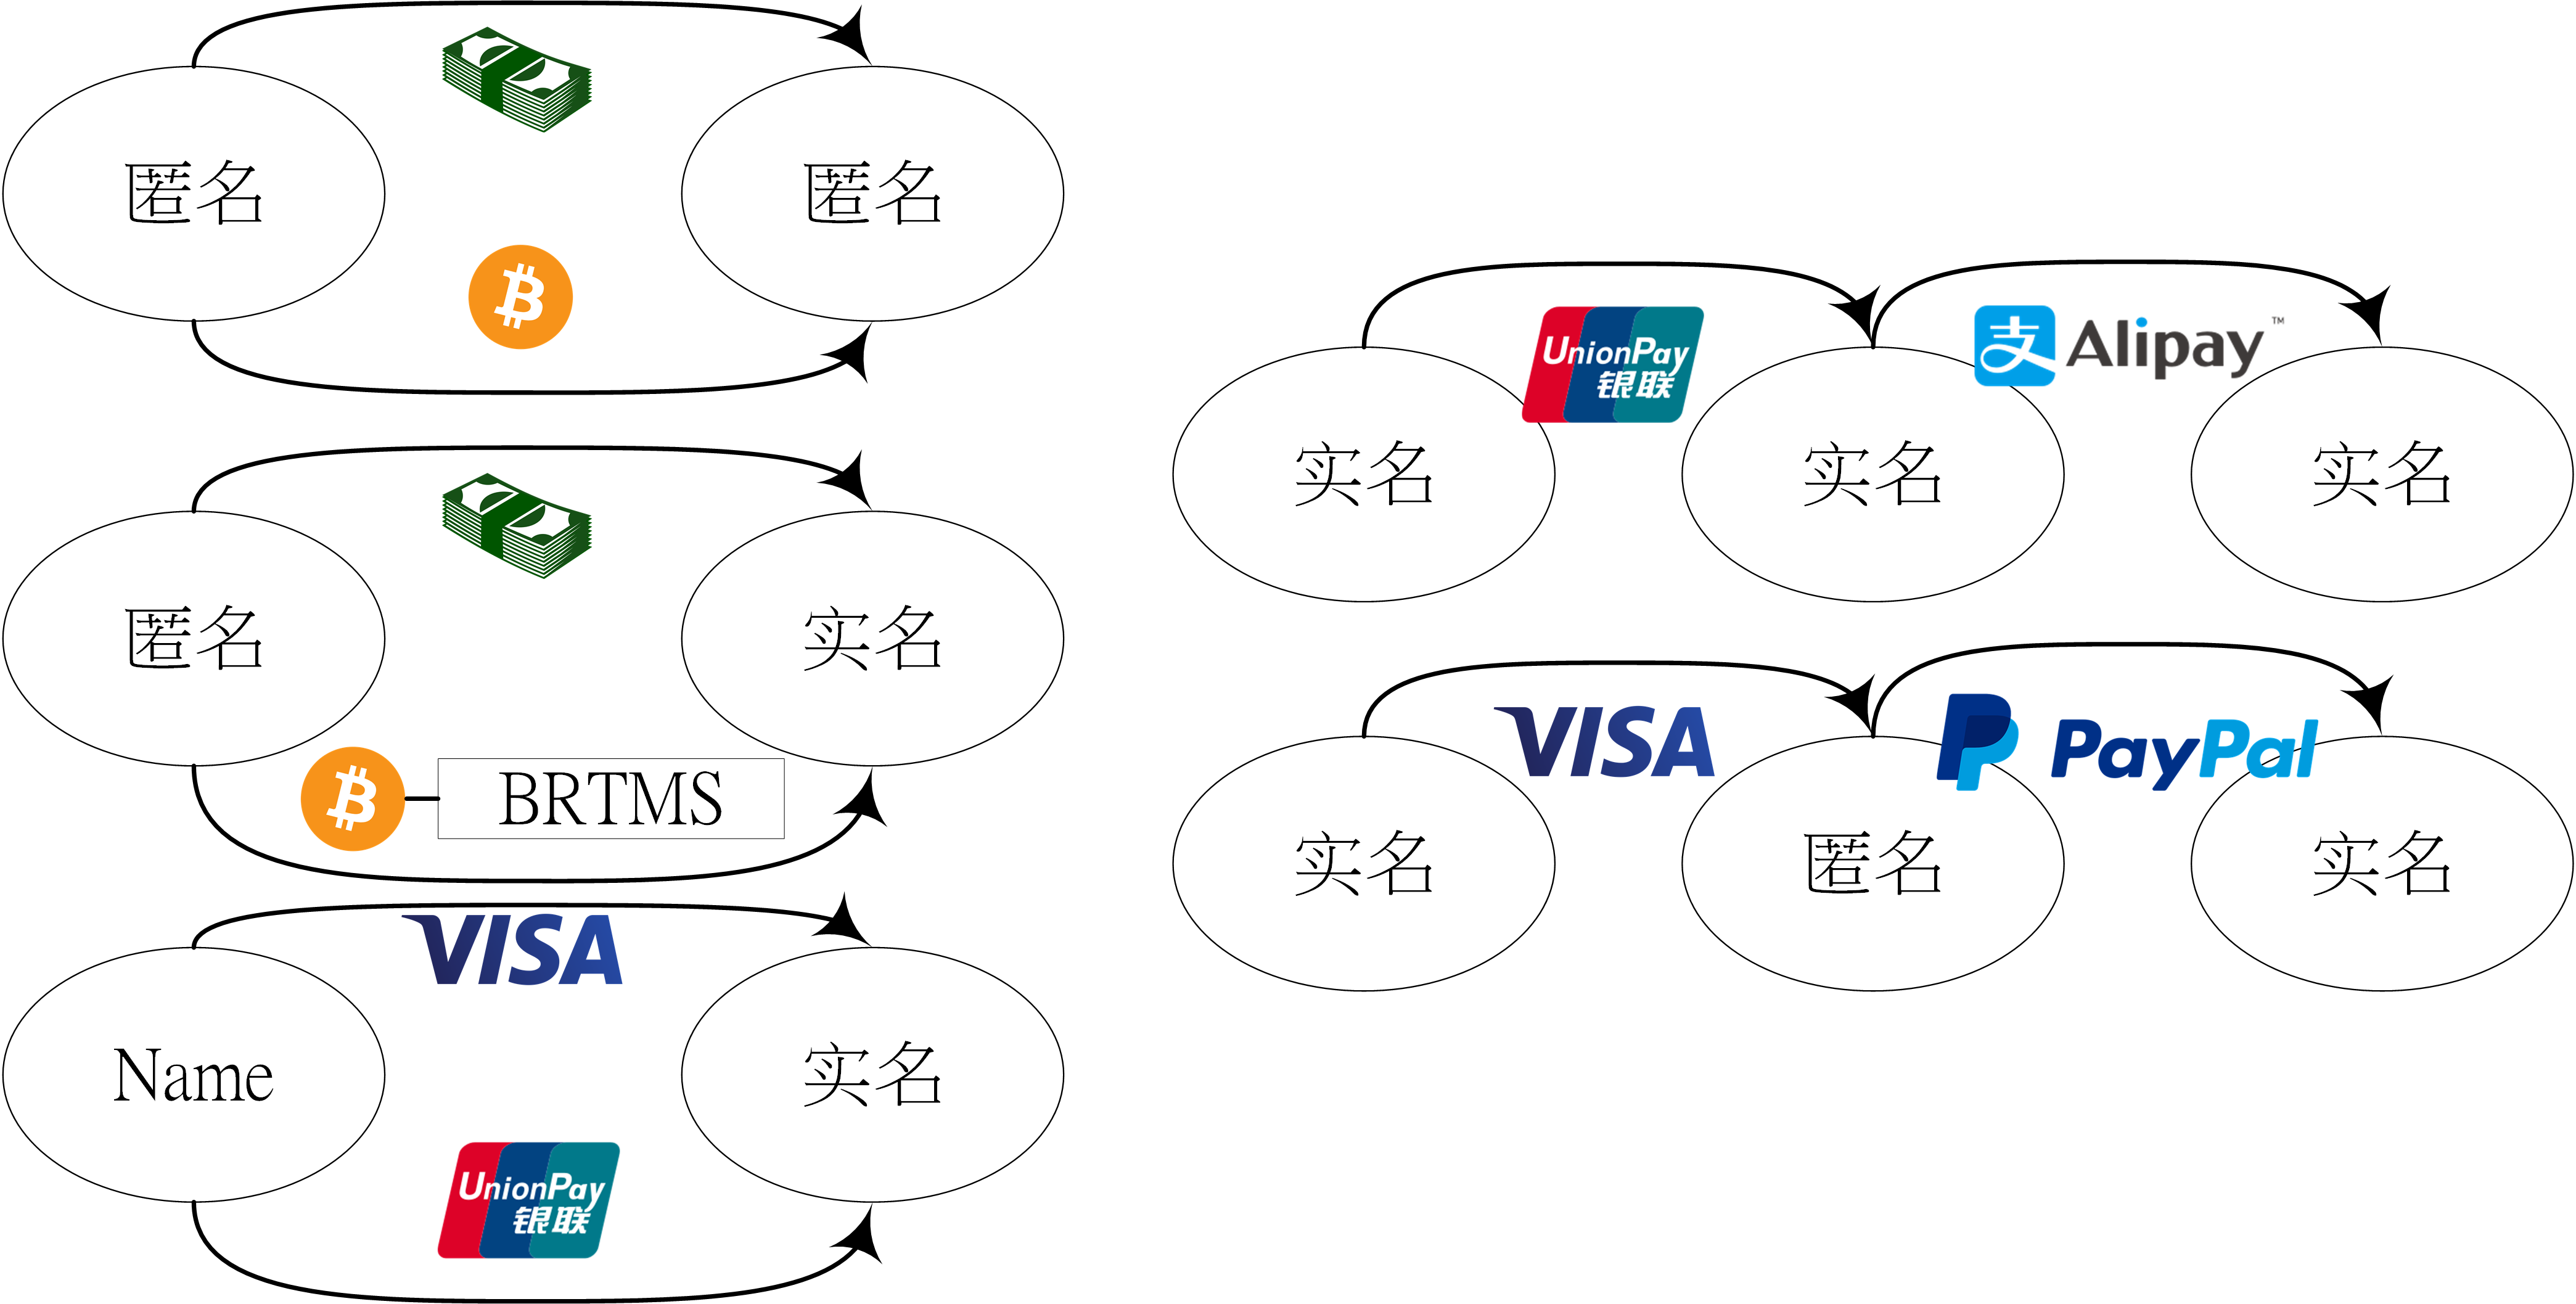
\includegraphics[width = 0.7\textwidth]{modeall.png}
	\caption{各種交易模型示意圖}\label{modeall}
\end{figure}

	\subsection{現金交易類型}
	在現金交易模型中大致分為匿名顧客支付匿名商家以及匿名顧客支付實名商家兩種,在過去的社會中,貝殼貨幣逐漸的被黃金取代,但黃金過於沈重在交易上相當不便。紙鈔漸漸取代⿈⾦,法定貨幣的概念因此形成。法定貨幣包括鈔票以及錢幣,在過往的法定貨幣存在著黃金價值支撐,使得法定貨幣具有價值,但經過歷史的變遷,已無⼤量的黃金作為法定貨幣的價值⽀撐,使法定貨幣漸漸地⾛向信⽤本位,紙鈔以及銅幣的使用皆不帶有持有者的真實姓名,因此在現金交易模型分析中將顧客支付皆歸類為匿名支付。

		\subsubsection{(一)匿名顧客支付匿名商家交易模型}
		現金法定貨幣的本身不存在使用者信息以及交易信息。現⾦是一種匿名的支付方式,早期有許多的商家並無向政府進行註冊,當顧客完成挑選商品進行結帳的同時,顧客只是將現金貨幣交付給商家,商家將商品賣給顧客,但在這過程中並無開立交易憑據。在商家無開立交易憑據的情況下,顧客完成此次的交易後,倘若該商品存在著瑕疵,進而引起商家與顧客之間的消費糾紛,使其在追溯的過程中存在沒有憑據的困擾。對於匿名顧客支付匿名商家可以保有顧客的信息隱私,但無法保障顧客應有的顧客權益。政府因沒有交易憑據而無法確認消費行為存在,使政府在課徵稅收的過程變得困難,且商家所販售的商品並無得到明確的信息紀錄,對於商家庫存管理只能依靠過去的經驗。對政府而言,商家販售的商品並無完整的商品信息,無法對商家商品進行安全性檢驗,使得國民購買的商品存在的許多安全疑慮。

		\subsubsection{(二)匿名顧客支付實名商家交易模型}
		現⾦最為常⾒的匿名顧客⽀付給實名商家交易模式,在匿名顧客以現⾦法定貨幣進⾏交易時,商家只要開⽴交易憑據,即被歸類為匿名顧客⽀付實名商家交易模型。商家在開⽴交易憑據的同時,憑據上所記載的信息包括職⼯信息、商家信息以及產品信息;職⼯信息記錄該筆交易的擔當人員,商家信息記錄商家與顧客建立交易行為的時間與地點,產品信息詳細記錄顧客於該商家購買的商品;交易憑據因此成為記錄交易事實的重要證明。對於顧客,因現⾦法定貨幣的匿名性使顧客依舊保有顧客信息隱私,但卻因為商家開⽴交易憑據得以保障顧客權益。商家因為開⽴交易憑據使商家為實名,因為實名使得商家可以經營品牌形象。除此之外,因為憑據記錄了產品信息讓商家在庫存管理以及收支計算變得更加容易。對政府⽽⾔,可以檢視商家的所得以及商家販售的商品,使政府可以更有效率的課徵稅收以及管理產品安全。

	\subsection{電子支付類型}
	電子商務的日趨盛⾏,電⼦支付交易模型也日漸普及,電子支付與加密貨幣的區塊鏈技術不同的是採用數據庫存儲著所有的交易信息,而用戶要能夠使用電子支付也必須接受電子支付運營商實名制的條件。在電子支付的數據庫中存在著黑客攻擊、信息不一致以及中心化運營的風險,但電⼦⽀付有效解決了難以現金支付遠距離之困境,也使得現今的網路購物變得更加發達。在電子支付交易模型中分為三種交易分別為實名顧客支付實名商家、實名顧客透過實名第三方再實名商家以及實名顧客透過匿名第三方再實名商家,以下將逐一說明。

		\subsubsection{(一)實名顧客支付實名商家交易模型}
		典型的實名顧客支付實名商家交易模式以VISA 國際電⼦⽀付公司為例,VISA 國際電⼦⽀付公司以下簡稱為VISA 公司,VISA 公司為中⼼化的運營,⽤⼾在使用VISA 電⼦⽀付以下簡稱為VISA 服務,前必須做詳盡的用戶真實⾝份認證,這使得VISA公司可以得到⽤⼾的所有信息,因此VISA公司擁有了允許或凍結相關⽤⼾⼾頭的使用權限,並且為了保護用戶隱私,所有的交易信息記錄皆被存儲在VISA 公司的數據庫當中。

		VISA公司透過不斷的優化電⼦⽀付技術已經可以接受每秒兩千筆的交易量,為了維持穩定的運營服務,VISA 公司對每筆交易收取固定⽐例的⼿續費。在使用VISA 服務的過程中,顧客因為必須進⾏實名驗證,使得顧客必須透露顧客個⼈信息,甚⾄可以針對這些個⼈信息進⾏商業上的交易。商家必須承擔VISA 服務所需的交易⼿續費,成本因此提高,使得商品售價必須做出相對應的調整。對政府⽽⾔,因為交易信息皆以中⼼化的⽅式存儲,可以⽅便的檢視,也可以快速的查閱商家收⼊課徵應繳的稅收。
		

		\subsubsection{(二)實名顧客透過實名第三方支付實名商家交易模型}
		電⼦⽀付⽅式⽇趨普及也使用戶可選擇的電⼦⽀付渠道更加多元,較為常⾒的包括VISA 電⼦⽀付以及銀聯電⼦⽀付,⽽每⼀家銀⾏為了讓用戶能在電⼦商務的⽀付上更為便利,會同時推廣電⼦⽀付,使得銀⾏卡⽀持電⼦⽀付,但更多的銀⾏卡林⽴使得用戶在卡⽚管理上更加繁瑣,第三⽅的支付整合平台開始出現成為解決⽅案。顧客可以先在實名第三⽅⽀付後台添加多張卡⽚,再以第三⽅⽀付統一進⾏付款。實名顧客透過實名第三⽅⽀付給實名商家時,顧客可以得到更⽅便的銀⾏卡管理,但卻在第三⽅⽀付上透露了個⼈交易信息,面對僅⽀持第三⽅⽀付的商家卻同時接受多家不同銀⾏卡的⽀付⽅式,政府僅需要調閱第三⽅⽀付公司就可查閱該公司所有⽤⼾的交易信息,且可更完整的採集到商家的收⼊信息。
		
		\subsubsection{(三)實名顧客透過匿名第三方支付實名商家交易模型}
		為了讓用戶可以保有更多的隱私,Paypal 公司提出了實名顧客透過匿名第三⽅⽀付實名商家的模式,顧客欲⽀付⼀筆款項給商家時,⾸先使⽤VISA 服務⽀付⼀筆資⾦到Paypal 公司,Paypal 公司再以Paypal 的名義⽀付該筆款項給商家。換⾔之,商家不會取得相關的顧客個⼈信息,也無法對顧客交易信息進⾏數據挖掘。值得⼀提的是,原本透過VISA 公司⽀付款項給商家,顧客就必須先負擔一筆的交易⼿續費給VISA 公司,而再透過Paypal 公司⽀付款項給商家時必須多經過Paypal 公司,顧客必須再⽀付第二筆交易⼿續費給Paypal 公司,這使得交易⼿續費更加的昂貴,但也因為多⼀個程序的資⾦轉移,使得顧客的個⼈信息可以得到隱匿。實名顧客透過匿名第三⽅⽀付實名商家的交易模型,對顧客⽽⾔商家可以開⽴交易憑據使得顧客保有顧客權益,同時也保有顧客的匿名性,但缺點是顧客必須承擔交易之間所增加的⼿續費;對於商家,可以透過交易信息管理商品庫存,快速計算商家的收益;而政府則可以快速地檢視商家交易信息以及商家所得。

		\subsection{交易比較}


		在上述兩種現金交易模型與三種電子支付模型中可以看出,初始的交易型態為匿名顧客⽀付匿名商家交易模式,因無法保障顧客與商家之間的權益而發展出匿名顧客⽀付實名商家交易模式,這使得顧客與商家之間可以兼顧雙⽅權益同時也保有顧客個⼈隱私,且可以讓政府快速地檢視稅務相關信息。

		⽀付技術的⽇新⽉異與VISA 公司的出現,使得電⼦商務可以快速的運⾏,但也因為VISA服務會透露太多的個⼈信息,顧客需求逐漸轉型成以實名顧客透過匿名第三⽅⽀付實名商家為基礎的交易模式,兼具以電⼦⽀付作為付款⽅式,且同時保有個⼈隱私。但其缺點是需要多經過⼀個資金轉移的程序,成為上述五種交易模型中交易手續費最為高昂的一種,但因其能保留顧客匿名性,讓透過匿名第三⽅⽀付的模式在電子支付類型中依然成為顧客的第一選擇。由上述分析可知,現⾦法定貨幣最佳的交易模型為匿名顧客⽀付實名商家交易模式,⽽電⼦⽀付類型的交易模式也趨向實名顧客透過匿名第三方支付給實名商家的方向演進。

		在使用加密貨幣作為交易貨幣的⽀付中,⼤部分的交易類型皆為如現⾦交易類型中匿名顧客⽀付匿名商家的交易模式,商家與顧客交易的過程中並無開⽴交易憑據,使得顧客與商家發⽣消費糾紛時因無法提出交易事實證明而無法擁有顧客權益保障。為了在使用加密貨幣時讓用戶可以同時兼顧顧客隱私與擁有顧客權益保障,也讓商家不需要⽀付運營商比過去更為高昂的⼿續費並能以公開匿名的⽅式檢視所有的交易信息,同時讓政府在課徵稅收的業務上可以更加便利,本⽂致⼒於設計出三者都能同時兼顧的加密貨幣交易系統。表\ref{txvs}為交易關係⽐較表。


		\begin{table}[!htbp]
		\centering
		\caption{交易關係比較表}
		\label{txvs}
		\begin{tabular}{|l|l|l|l|l|}
		\hline
		 & 顧客 & 仲介單位 & 商家 & 商品 \\ \hline
		現金 & 匿名 & 無 & 匿名/實名 & 匿名/實名 \\ \hline
		VISA & 實名 & 無 & 實名 & 實名 \\ \hline
		支付寶 & 實名 & 實名 & 實名 & 實名 \\ \hline
		PayPal & 實名 & 匿名 & 實名 & 實名 \\ \hline
		加密貨幣 & 匿名 & 無 & 匿名/實名 & 匿名/實名 \\ \hline
		\end{tabular}
		\end{table}

\section{功能性需求分析}

在現今的加密貨幣交易系統中採用匿名對匿名⽀付的交易模式,這樣的交易模式顧客無法擁有權益保障,商家需支付高昂的交易手續費,政府也無法在交易中課徵稅收。傳統交易模式中所採用實名⽀付給實名的交易模式雖然可以有效地保障顧客權益,但在這對顧客個⼈隱私⽇趨重視的世代中,個⼈信息越來越有價值,個⼈信息的保護更是成為重要的課題。在本系統中,將以加密貨幣-⽐特幣為基礎,設計⼀個以匿名顧客⽀付給實名商家為基礎的比特幣交易監督系統。在實現匿名⽀付給實名的交易模型同時,也將商家的庫存信息同時加⼊,使商家也可以輕鬆地使用本系統管理產品庫存。如圖\ref{UC}所示,在本系統中,參與者總共有三種,分別為商家、職⼯以及顧客。

商家,在本系統中為第⼀個參與者,因為必須要有商家的註冊參與,才可以進⼀步的添加職⼯以及商家產品信息,如此⼀來商家才有商品可以販售。參與者商家本⾝有三項需求,分別為⽤⼾註冊與登⼊、職⼯管理以及商家產品管理。以下將逐⼀說明:


	\begin{enumerate}
	\item 用戶註冊與登入:為了得到政府的認證,商家必須接受政府的檢視,提交相關的信息到本系統中。在用戶註冊的頁面當中,進行用戶的註冊或是登入都需要用戶信息,因此需要包括加載用戶信息。
	\item 職工管理:在完成用戶註冊與登入之後,才得以進行職工管理,商家本身會有大於或等於一個職工的帳號,商家的註冊者本身會是一個職工。在職工管理當中,需要有查詢職⼯帳⼾與修改職⼯帳⼾兩項功能,查詢職工帳戶的功能必須包括加載職工信息。在進行職工帳戶修改時需要包括職工信息以及商家信息,才得以對職工信息進行修改。
	\item 商家產品管理:商家需要添加產品信息至商家產品信息中,產品為政府認可的產品認證編號,在本系統中產品本身不存在價格,需要參與者商家將產品添加至商家產品信息中才可以添加價格,這樣的設計可以讓不同的商家在不同的產品設置不同的價格。除了商家對商家產品價格需求,同時也需要對產品庫存進行管理,透過區塊鏈加密貨幣公開交易信息的特性,可以使得庫存管理以及交易信息更快速地核對。在商家產品管理中需要查詢產品信息,在查詢產品信息的同時包括加載產品信息,使得查詢過程可以順利運作。在查詢完成產品信息後,商家需要將產品信息與商家信息添加到商家產品信息當中,在這過程中需要包括加載商家信息以及商家產品信息。

	\end{enumerate}

職⼯,需要進⾏⽤⼾註冊並且通過政府的審查,在完成審查之後需要進⼊商家交易管理建置移動收銀機。參與者職⼯本⾝有兩項需求,分別為⽤⼾註冊與登⼊、及商家產品管理。以下將逐⼀說明:


	\begin{enumerate}
	\item 用戶註冊與登入:要成為職工之前職工需要進行用戶註冊,等待政府的審查之後,並經由商家進行職工管理將用戶與商家一併提交到職工信息,才得以成為正式的職工,職工的用戶註冊與登入皆需要包括加載用戶信息,才能使得註冊與登入功能順利運行。
	\item 商家交易管理:在完成登入後,商家交易管理將會加載相關信息,包括加載職工信息,在交易信息中添加職工編號,加載商家信息使得在進行交易的過程中可以將商家的比特幣地址傳送給顧客等待接收款項以及加載商家產品信息使得職工的移動設備上可以顯示所有的商家產品信息,在完成信息加載後職工的移動裝置已經成為一台移動收銀機。在職工在進行掃碼的過程會創建交易清單並且將交易清單傳送給顧客等待顧客的付款。在等待付款時,商家交易管理需要認證該筆交易是否有效,因此需要加載交易信息,
	\end{enumerate}

顧客,為了保持顧客的身份匿名,參與者顧客與參與者職工和商家不同,顧客在參與本系統的同時不需要註冊帳戶以及登入用戶帳戶,顧客主要需求為加載過去與顧客相關的交易信息,以及使用比特幣支付進行付款:


顧客交易管理:顧客需要加載交易信息,但因為交易信息中的信息並無詳細闡述商家產品信息,因此需要進一步加載商家產品信息使得交易明細更加的清楚。除了顯示過去的交易信息的需求,顧客更需要創建一筆交易以⽐特幣進⾏付款。待付款完成之後,等待參與者商家向顧客回覆⽀付完成即確立該筆交易完成。

	\begin{figure}[!htbp]
	\centering
	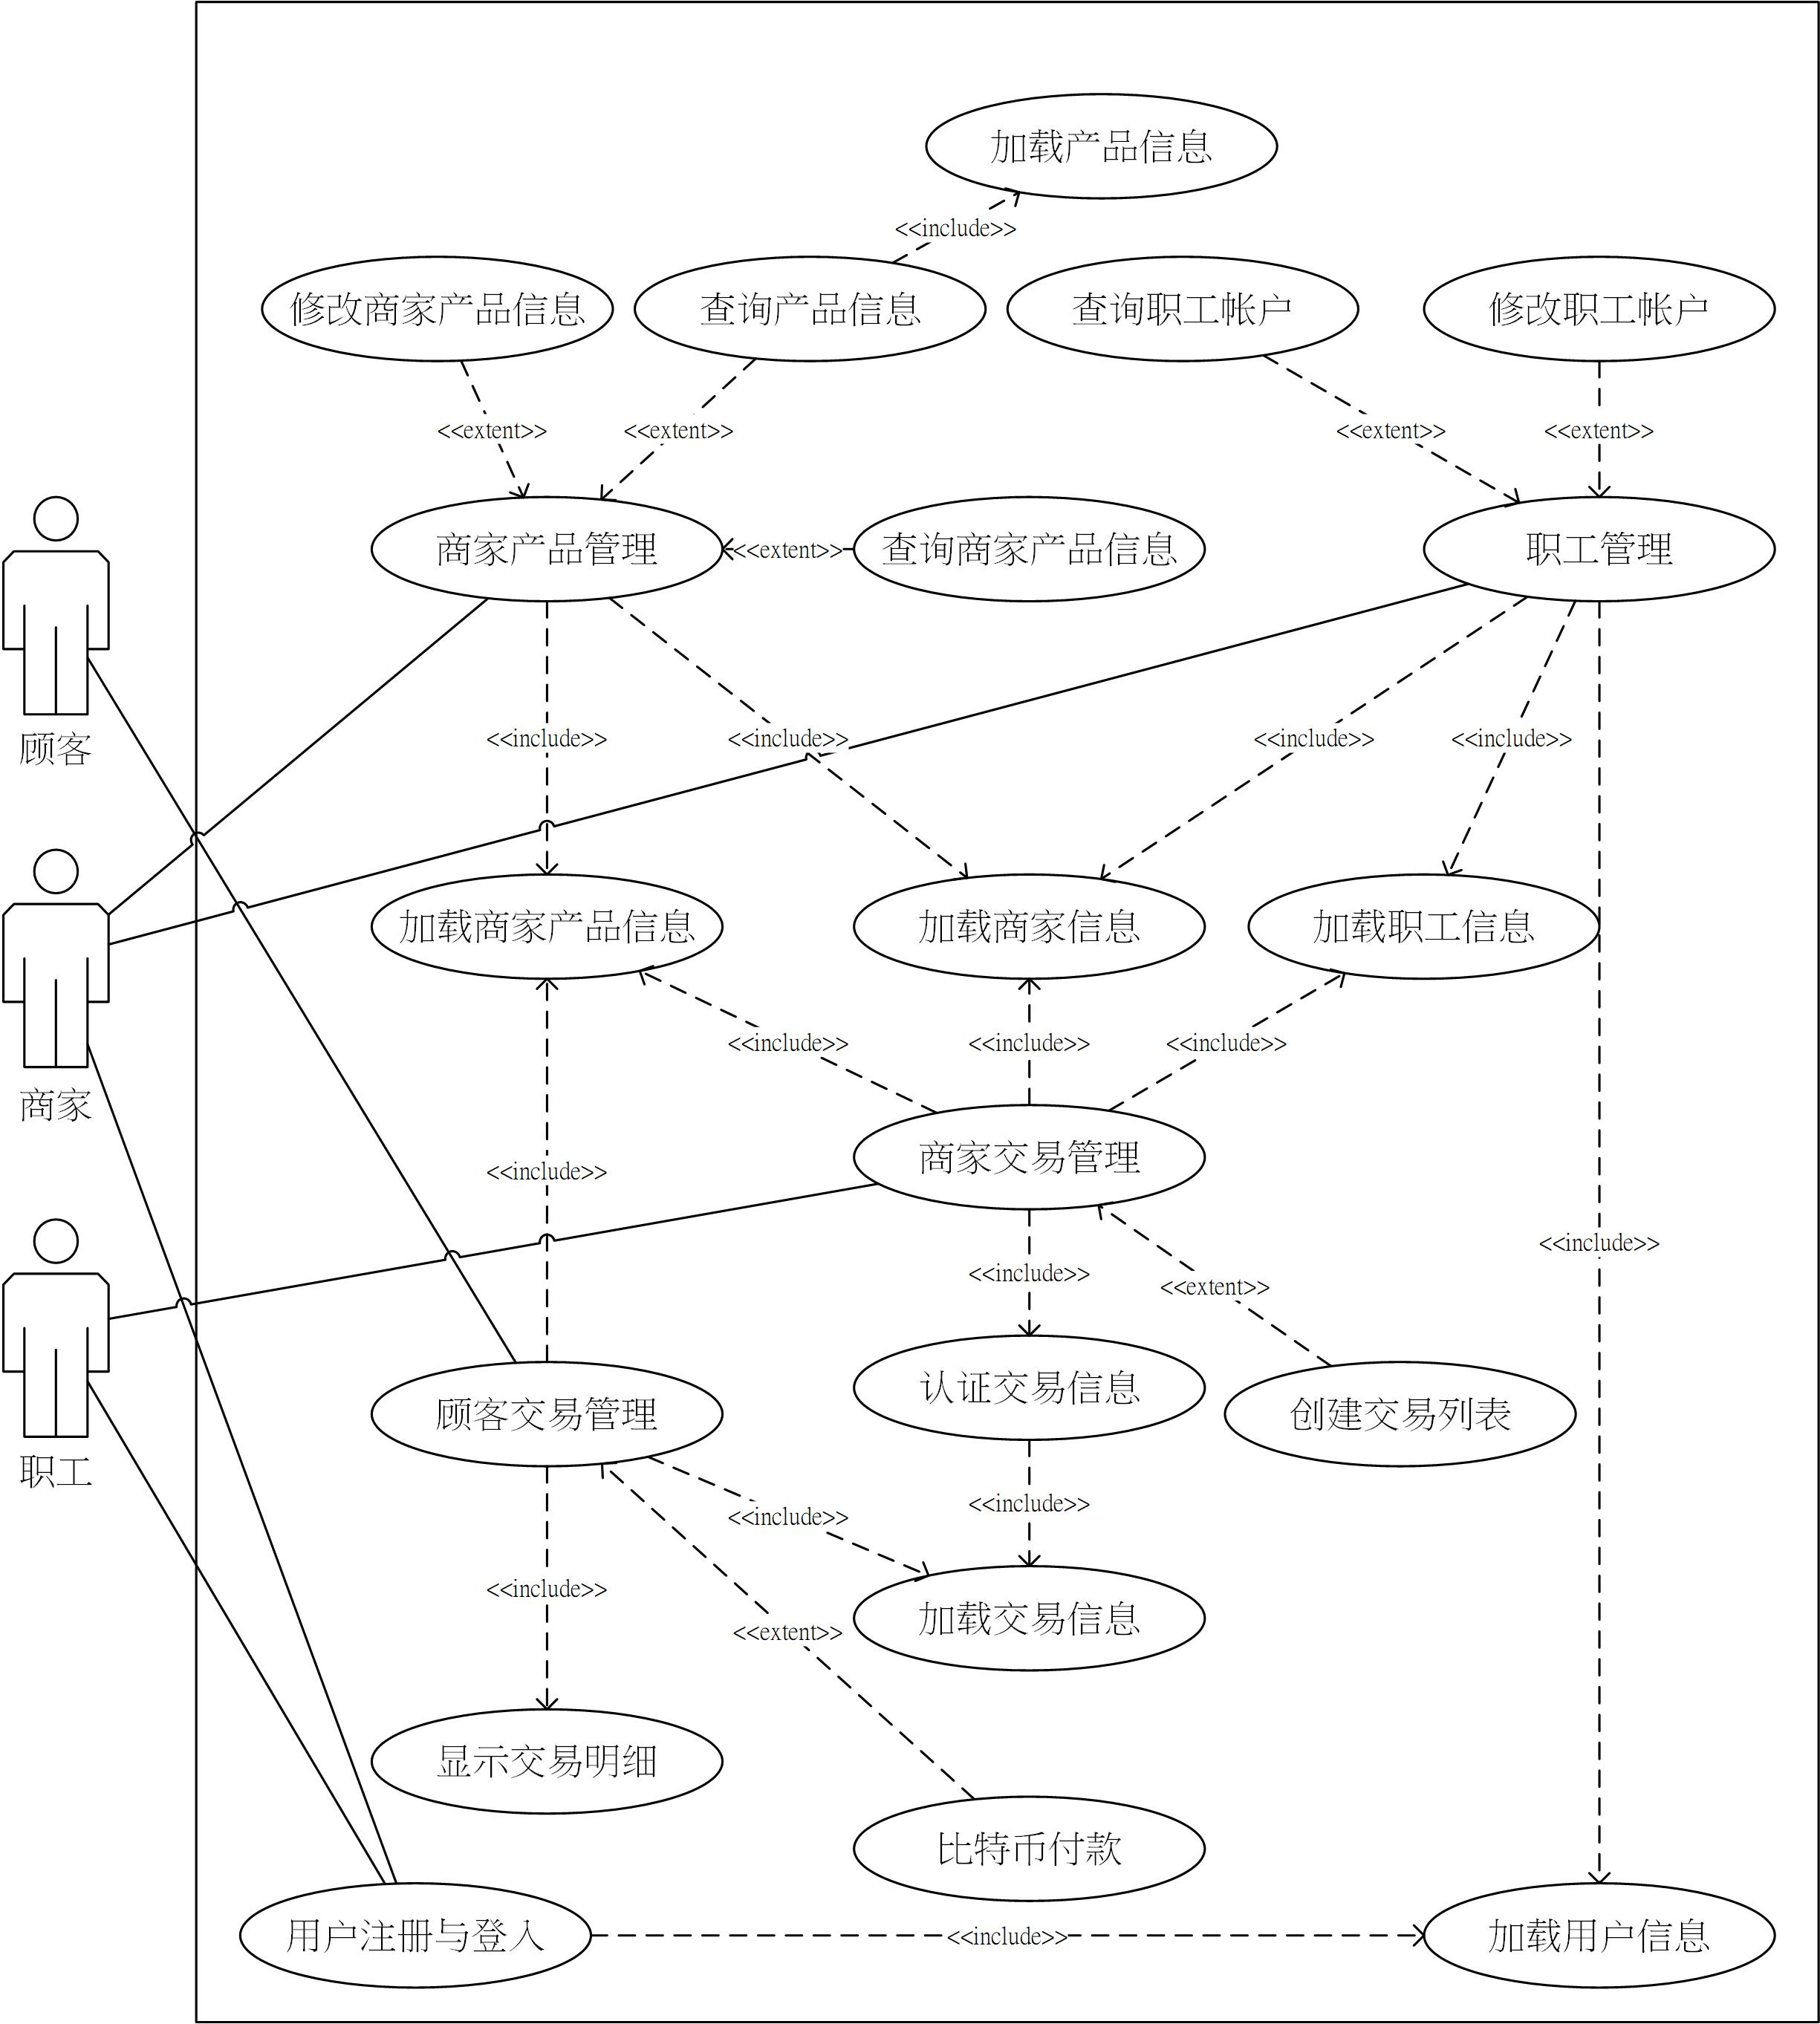
\includegraphics[width = 0.9\textwidth]{UC.jpg}
	\caption{比特幣交易監督系統⽤例圖}\label{UC}
	\end{figure}

	\section{非功能性需求分析}

	\subsubsection{(一)性能需求}
	
	本文所實踐之系統為比特幣的交易监督系统,參與者商家需要使用到商家端建置與管理商品資訊子系統,在參與者商家操作該子系統時,系統在設置完成後,於存儲的過程中應於三秒內完成。於商家端建置與管理商品資訊子系統、商家端行動收銀與交易明細系統應達到於兩秒內完成子系統與數據庫之間的信息傳遞以及信息存儲,倘若商家與顧客在完成交易後,卻無法得到快速的系統響應,這使得參與者顧客與職工收到⽀付完成的回覆,甚至導致商家的交易塞車影響用戶的消費體驗。

	\subsubsection{(二)可拓展性}

	本論文提出的系統為比特幣的交易监督系统雛形,於系統設計中將優先考慮最必要功能並加以實現,包括商家端建置與管理商品資訊子系統、商家端行動收銀與交易明細系統以及顧客端行動支付與交易明細系統,於上述三個子系統中皆可以進行數據庫欄位的添加,使得交易信息、商家信息、商品信息、商家產品信息、用戶信息以及職工信息更加的完備且更符合實際上業務需求。在未來甚⾄可以加⼊更完整的稅務信息,使政府在稅務計算⽅⾯可以大幅降低⼈⼒資源成本且更快速地進⾏稅務統計,而庫存管理⽅⾯可以加⼊庫存預測的服務。

	\subsubsection{(三)可操作性}
	在本系統中的三個⼦系統中,為了將商家端⾏動收銀與交易明細系統,以及顧客端⾏動⽀付與交易明細系統實現在⼿持移動裝置Android 操作系統上,於介⾯設計⽅⾯應給予商家⽤⼾以及顧客⽤⼾⼈性化的操作交互設計,以及於代碼撰寫⽅⾯應更加簡潔,使得⽤⼾在啟動本⼿持移動端應⽤程序時可以在最短的時間內完成初始化程序加載。除了針對⽤⼾交互⽅⾯的優化,也需要添加各個功能項⽬的使⽤說明,以及⽤⼾操作問題反饋,給予使用本系統的移動設備在應⽤程序上能快速的修正以提升⽤⼾體驗。商家端建置與管理商品資訊⼦系統是以Java 編程語⾔實現,針對參與者商家操作進⾏設計,該⼦系統需簡單明確的呈現商家信息、產品信息以及商家產品信息,使參與者商家可以快速地檢視所有商品,並新增、修改以及刪除相關產品信息,包括價格、庫存以商家產品描述。

	\subsubsection{(四)軟件與硬件環境需求}
	表\ref{eva}為本文提出系統的軟件與硬件環境需求,商家交易客戶端與顧客交易客戶端是建置在Android手機的應用程序,本文提出的交易方式為比特幣,因此導入bitcoinj\supercite{Bitcoinclients}對比特幣錢包進行管理,該套件可以生成比特幣地址、同步比特幣區塊鏈、透過AES加密算法保護比特幣錢包以及發起比特幣交易至比特幣網路。針對數據庫的控制數據傳輸選用JDBC\supercite{JDBCdatabaseaccesswithJava:atutorialandannotatedreference}實現數據庫的新增、修改、刪除以及查詢的功能,商家交易客戶端與顧客交易客戶端的手機移動裝置必須要內置NFC傳感器用來傳送與接收交易信息。商家管理客⼾端是以Java 編程語⾔實現,軟件環境中需⽀持Java ⼯作環境,服務器端則需要SQL 環境進行數據庫搭建。


	\begin{table}[!htbp]
	\centering
	\caption{環境需求表}
	\label{eva}
	\begin{tabular}{|c|c|c|c|}
	\hline
	- & 操作系統 & 軟件 & 硬件 \\ \hline
	\begin{tabular}[c]{@{}c@{}}商家交易\\ 客戶端\\ 與\\ 顧客交易\\ 客戶端\end{tabular} & \begin{tabular}[c]{@{}c@{}}Android 4 \\ 或以上\end{tabular} & \begin{tabular}[c]{@{}c@{}}Java 7 或以上 \\ bitcoinj v0.14.6 \\ JDBC 4.2 或以上\\  Maven 3+\end{tabular} & \begin{tabular}[c]{@{}c@{}}存儲容量:32GB\\ 內存容量:2GB\\ 網路需求:10兆或以上\\ 傳感器:NFC傳感器\end{tabular} \\ \hline
	\begin{tabular}[c]{@{}c@{}}商家管理\\ 客戶端\end{tabular} & \begin{tabular}[c]{@{}c@{}}Windows 7 \\ 或以上\end{tabular} & \begin{tabular}[c]{@{}c@{}}Java 7 或以上 \\ JDBC\end{tabular} & \begin{tabular}[c]{@{}c@{}}硬盤容量:100GB\\ 內存容量:4GB\\ 處理器:Core 2 Duo 或以上\\ 網路需求:10兆或以上\end{tabular} \\ \hline
	服務器端 & \begin{tabular}[c]{@{}c@{}}Windows Server \\ 2003 \\ 或以上\end{tabular} & \begin{tabular}[c]{@{}c@{}}Microsoft SQL Server \\ bitcoin-qt 0.8.X 或以上 \\ Apache HTTP Server\end{tabular} & \begin{tabular}[c]{@{}c@{}}硬盤容量:1000GB\\ 內存容量:16GB\\ 處理器:Xeon E3 或以上\\ 網路需求:100兆或以上\end{tabular} \\ \hline
	\end{tabular}
	\end{table}




%		\begin{figure}[!htbp]
%			\centering
%			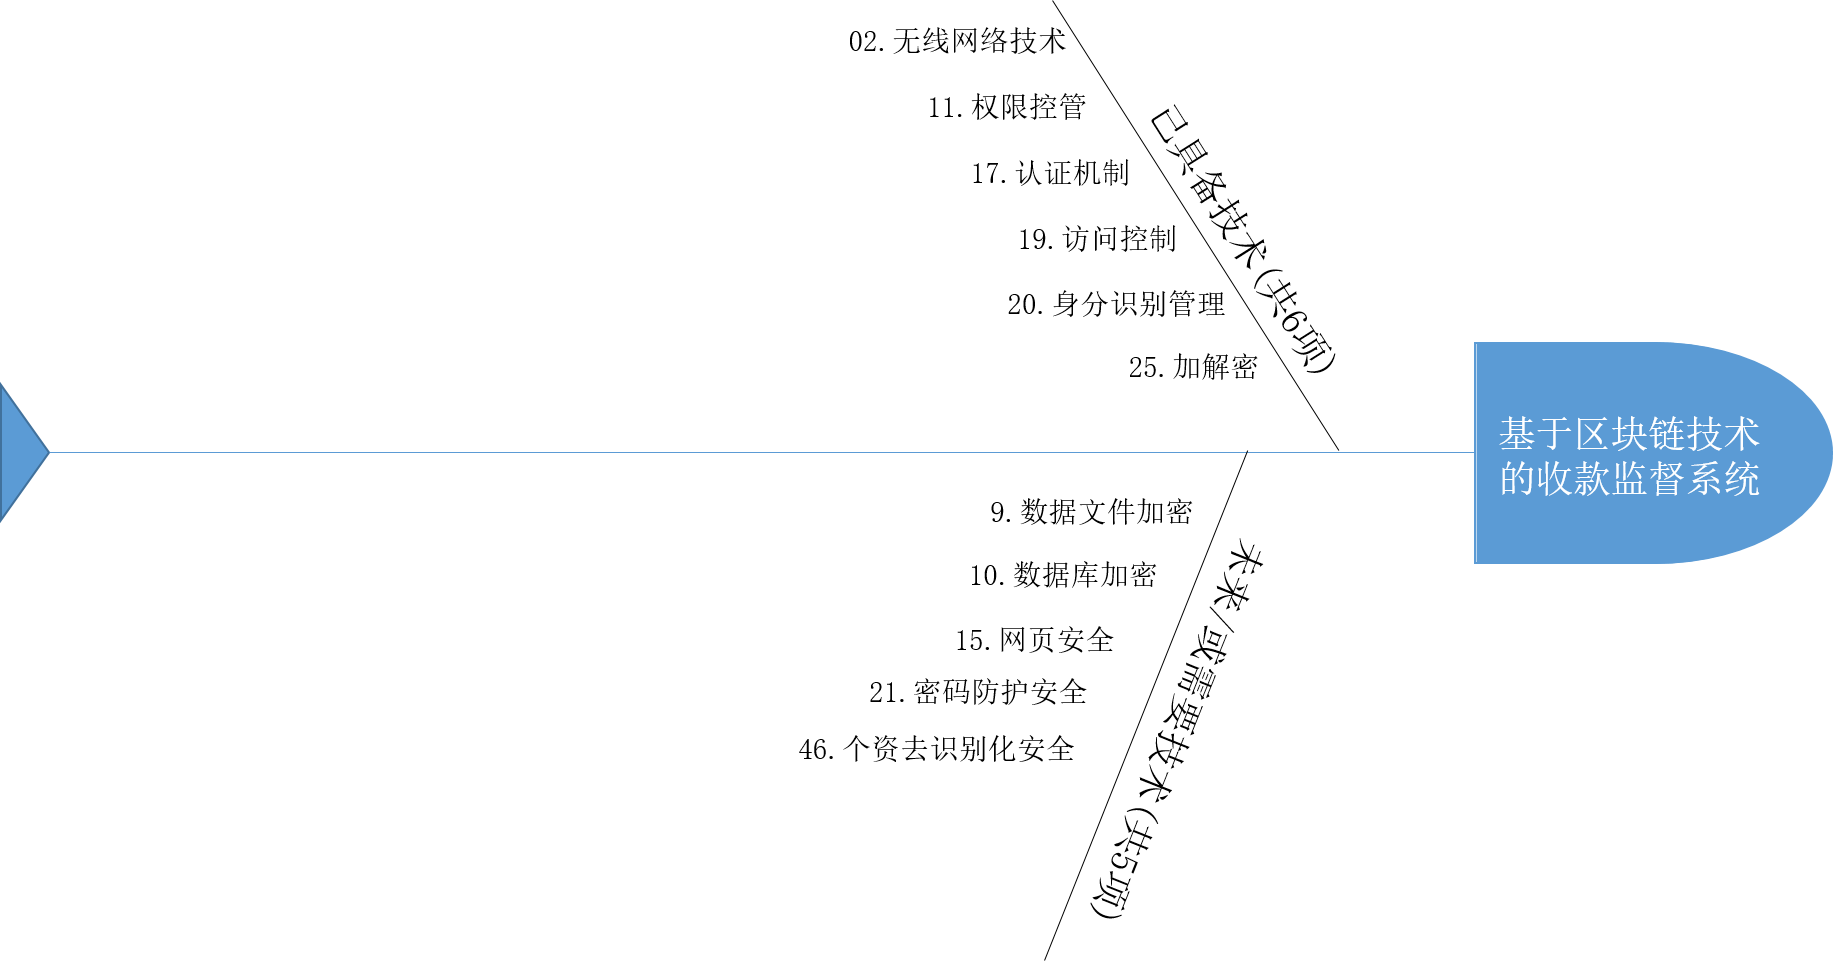
\includegraphics[width = 1\textwidth]{fish2.png}
%			\caption{魚骨圖(2)}\label{fish1}
%		\end{figure}

%		\subsection{匿名顧客對匿名商家}
%	\section{各種交易模型比較}
